    \chapter{راهنمای استفاده از کلاس \lr{\protect\ttfamily \lowercase{thesis-qom}}}
    \section{مقدمه}
    حروف‌چینی پایان‌نامه/رساله یکی از موارد پرکاربرد استفاده از تِک/لاتِک در بین دانشجویان و شاید نقطه شروع آشنایی ایشان با این سیستم بی‌نظیر است. 
    خوب از آنجایی که نگارش باید به زبان پارسی باشد، یکی از بهترین انتخاب‌ها، زی‌پرشین است. علاوه بر پایان‌نامه/رساله امکان حروفچینی نامه، 
    مقاله، پوستر و حتی ارائه نیز با زی‌پرشین مقدور است. از طرفی، یک  پایان‌نامه/رساله،  احتیاج به تنظیمات زیادی از نظر صفحه‌آرایی  دارد 
    تا مطابق با نظر تحصیلات تکمیلی موسسه مطبوع گردد و همین ممکن است برای
    یک کاربر مبتدی، کمی مشکل باشد. گرچه غالب کاربران تا کنون بارها بارها از نرم‌افزار مایکروسافت ورد استفاده کرده‌اند لکن به جرات 
    می‌توان گفت که بیشتر آنان از زمره کاربران عادی این نرم‌افزار هستند و توانایی حروفچینی حرفه‌ای با آن را ندارند. به همین سبب برخی موسسات 
    اقدام به تهیه یک قالب آماده ورد برای دانشجویان می‌نمایند ولی متاسفانه این قالب معمولاً برای یکی از نسخه‌های ورد تهیه می‌شود و در دیگر نسخه 
    به درستی عمل ننموده و دانشجویان را به دردسر می‌اندازد؛ از طرف دیگر لاتک چنین محدودیتی ندارد و کاربران به راحتی می‌توانند از کیفیت خروجی 
    مطمئن بوده و بدون هیچ نگرانی، تنها به متن خود بپردازند. 
    به همین دلایل، برای راحتی کار کاربر، کلاس حاضر با نام 
     \LRE{\Verb!thesis-qom!}
     برای حروف‌چینی پروژه‌ها، پایان‌نامه‌ها و رساله‌های دانشگاه قم با استفاده از نرم‌افزار زی‌پرشین،  آماده شده است. این فایل به 
    گونه‌ای طراحی شده است که کلیه خواسته‌های مورد نیاز  مدیریت تحصیلات تکمیلی دانشگاه قم را برآورده می‌کند. همچنین حروف‌چینی بسیاری
    از قسمت‌های آن، به طور خودکار انجام می‌شود.

    کلیه فایل‌های لازم برای حروف‌چینی با کلاس گفته شده، داخل پوشه‌ای به نام
     \LRE{\Verb!thesis-qom!}
      قرار داده شده است. توجه داشته باشید که برای استفاده از این کلاس باید فونت‌هایی که در پوشه \Verb+fonts+ قرار دارد روی 
        روی سیستم شما نصب شده باشد. این پوشه شامل فونت‌های ذیل است:‌
        \begin{enumerate*}
            \item \Verb+Yas+
            \item \LR{\Verb+XB Niloofar+}
             \item \Verb+IranNastaliq+
            \item \Verb+IRLotus+
            \item \LR{\Verb+XB Zar+}
            \item \LR{\Verb+XB Titre+}
        \end{enumerate*}
        
    \section{این همه فایل؟!}\label{sec2}
    از آنجایی که یک پایان‌نامه یا رساله، یک نوشته بلند محسوب می‌شود، لذا اگر همه تنظیمات و مطالب پایان‌نامه را داخل یک فایل قرار بدهیم، باعث شلوغی
    و سردرگمی می‌شود. به همین خاطر، قسمت‌های مختلف پایان‌نامه یا رساله  داخل فایل‌های جداگانه قرار گرفته است. مثلاً تنظیمات  کلاس داخل فایل
    \LRE{\Verb!settings.tex!}، 
    مطالب فصل اول، داخل \linebreak
    \Verb!chapter1!
    و ... قرار داده شده است. نکته مهمی که در اینجا وجود دارد این است که از بین این  فایل‌ها، فقط فایل 
    \LRE{\Verb!thesis.tex!}
    قابل اجرا است. یعنی بعد از تغییر فایل‌های دیگر، برای دیدن نتیجه تغییرات، باید این فایل را اجرا کرد. بقیه فایل‌ها به این فایل، کمک می‌کنند تا بتوانیم خروجی کار را ببینیم. اگر به فایل 
    \LRE{\Verb!thesis.tex!}
    دقت کنید، متوجه می‌شوید که قسمت‌های مختلف پایان‌نامه، توسط دستورهایی مانند 
    \Verb!input!
    و
    \Verb!include!
    به فایل اصلی، یعنی 
    \LRE{\Verb!thesis.tex!}
    معرفی شده‌اند. بنابراین، فایلی که همیشه با آن سروکار داریم، فایل 
    \LRE{\Verb!thesis.tex!}
    است.
    در این فایل، فرض شده است که پایان‌نامه/رساله، شامل چند فصل و پیوست است. با این حال، اگر
      پایان‌نامه/رساله، به فصول یا پیوست‌های بیشتر نیاز دارد، باید خودتان فصل‌های بیشتر را به این فایل، اضافه کنید. این کار، بسیار ساده است. فرض کنید بخواهید یک فصل دیگر هم به پایان‌نامه، اضافه کنید. برای این کار، کافی است یک فایل با نام 
    \Verb!chapterN!  --\lr{N} شماره فصل بعدی--
    و با پسوند 
    \Verb!.tex!
    بسازید و آن را داخل پوشه 
    \LRE{\Verb!thesis-qom!}
    قرار دهید و سپس این فایل را با دستور 
    \Verb!\include{chapterN}!
    داخل فایل
    \LRE{\Verb!thesis.tex!}
    و بعد از آخرین دستور
    \Verb!\include!
    و قبل از \Verb+\appendix+ قرار دهید. حال اگر می‌خواهید یک پیوست دیگر بیفزایید باید آن را پس از آخرین \Verb!\include! 
    که بعد از \Verb+\appendix+ آمده است قرار دهید. 

    \section{از کجا شروع کنم؟}
    قبل از هر چیز، بدیهی است که باید یک توزیع تِک مناسب مانند 
    \Verb!Live TeX!
    و یک ویرایش‌گر تِک مانند
    \Verb!Texmaker!
    را روی سیستم خود نصب کنید.  نسخه بهینه شده \Verb!Texmaker!  را می‌توانید  از سایت 
     \href{http://www.parsilatex.com}{پارسی‌لاتک}%
    \LTRfootnote{\url{http://www.parsilatex.com}}
     و \Verb!Live TeX!  را هم می‌توانید از 
     \href{http://www.tug.org/texlive}{سایت رسمی آن}%
    \LTRfootnote{\url{http://www.tug.org/texlive}}
     دانلود کنید و یا آن را از طریق 
     \href{http://parsilatex.com/site/?p=185}{فروشگاه سایت پارسی‌لاتک}%
    \LTRfootnote{\url{http://parsilatex.com/site/?p=185}}
     به همراه مجموعه‌ای غنی از مثال، کتاب و فیلم آموزشی تهیه نمایید. برای توضیحات بیشتر به پیوست~\ref{chap:installation} مراجعه نمایید. 
     
    در مرحله بعد، سعی کنید که  یک پشتیبان از پوشه 
    \LRE{\Verb!thesis-qom!}
     بگیرید و آن را در یک جایی از هارددیسک سیستم خود ذخیره کنید تا در صورت خراب کردن فایل‌هایی که در حال حاضر، با آن‌ها کار می‌کنید، همه چیز را از 
     دست ندهید. البته برای گرفتن یک پشتیبان روی فضای اینترنت می‌توانید از 
     \href{https://www.dropbox.com/}{دراپ‌باکس}%
    \LTRfootnote{\url{https://www.dropbox.com/}}
      و یا 
      \href{https://github.com}{گیت‌هاب}%
    \LTRfootnote{\url{https://github.com}}
       استفاده نماید تا هر زمان که به کامپیوتر خود 
     دسترسی نداشتید نیز بتوانید براحتی از طریق وب، فایل‌هایتان را بررسی نمایید؛‌ البته پشیتبان‌گیری روی اینترنت محدود به گزینه‌ها نبوده و دانشجویان 
     می‌توانند  خدمات دیگری اعم از رایگان یا پولی را بکار برند. 
     
     \subsection{ مشخصات پایان‌نامه/رساله}
    بعد از موارد گفته شده، فایل 
    \LRE{\Verb!settings.tex!}
    را باز کنید و مشخصات پایان‌نامه خود مثل نام، نام خانوادگی، عنوان پایان‌نامه و ... را جایگزین مشخصات موجود در فایل
     کنید. هر چند که شاید نیاز به ایجاد یک فایل مجزا برای اینکار نبود لکن همانطور که در بخش~\hbox{\ref{sec2}} شرح داده شد با اینکار، سعی داریم که فایل 
     اصلی، \Verb!thesis.tex!، تنها نشان دهندهٔ ساختار محتوایی پایان‌نامه/رساله شما باشد. 
     در  فایل \Verb!settings.tex! دستوری به نام \Verb+\thesisdetails+ وجود دارد که تمامی پارامترهای لازم از طریق این دستور تنظیم می‌شود. 
     دقت داشته باشید که نیازی نیست 
    نگران چینش این مشخصات در فایل پی‌دی‌اف خروجی باشید. فایل     \LRE{\Verb!thesis-qom.cls!}
    همه این کارها را به طور خودکار برای شما انجام می‌دهد. در ضمن، موقع تغییر دادن دستورهای داخل فایل
    \LRE{\Verb!settings.tex!}
     کاملاً  دقت کنید. این دستورها، خیلی حساس هستند و ممکن است با یک تغییر کوچک، موقع اجرا، خطا بگیرید. برای دیدن خروجی کار، فایل 
     را     \Verb!Save!،     (نه     \Verb!As Save!)    کنید و بعد به فایل 
    \LRE{\Verb!thesis.tex!}
    برگشته و آن را اجرا کنید.
    
    همانطوری که تاکنون با نگاه به فایل \LRE{\Verb!settings.tex!} متوجه شده‌اید، تمامی تنظیمات لازمه درون دستوری به نام \Verb+\thesisdetails+ 
    قرار دارد و برای مقداردهی کافی است مقدار مطلوب پس از علامت \Verb+=+ که بعد از نام فیلد مورد نظر آمده است درج گردد؛‌ توجه نمایید که 
    اگر مقدار فیلد مطلوب بیش از یک خط به خود اختصاص می‌دهد این مقدار باید بین آکولاد باز و بسته محصور گردد و یا اینکه محتویات مطلوب 
    در فایلی جداگانه نوشته شده و سپس در جلوی آن فیلد با دستورات \Verb+\input+  و یا \Verb+\include+ وارد گردد. 
    جداکننده بین فیلدها کاراکتر کامای لاتین است؛ دقت نماید که به اشتباه کاراکتر ویرگول فارسی را بکار نبرید. 

    فیلدها در دو دسته فارسی و لاتین تعریف شده‌اند که نام خود فیلد گویا بوده و نیاز به توضیح اضافی ندارد. فیلدهای فارسی تعریف‌شده 
    در جدول~\ref{tab:persianfields} آمده است. تنها نکته‌ای که باید در نظر داشته باشید این است که در فرم دفاع در جلوی نام اساتید مرتبه 
    علمی آن‌ها نیز نوشته خواهد شد لذا برای مشخص نمودن مرتبه علمی استاد مورد نظر باید مرتبه ایشان را داخل پرانتز جلوی نام ایشان بنویسید، همانند 
    \fbox{دکتر اکبر طیبی (دانشیار)}. 
    نکته فوق شامل «نماینده تحصیلات تکمیلی» نیز می‌گردد. فیلدهای لاتین نیز در جدول~\ref{tab:latinfields} آمده است. دقت نمایید که تمامی 
    فیلدهای لاتین با حروف کوچک نگاشته شده‌اند و تغییر حالت هر یک از حروف این فیلدها سبب بروز خطا می‌گردد. 
    
\begin{table}[htb]
\caption{فیلدهای فارسی قالب پایان‌نامه/رساله تعریف شده در دستور \lr{\textbackslash{}thesisdetails}}
\label{tab:persianfields}
\smallskip
\hrule\hrule
\begin{multicols*}{3}
    \begin{enumerate}
        \item نام و نام‌خانوادگی
        \item شماره دانشجویی
        \item عنوان
        \item دانشکده
        \item گروه
        \item رشته
        \item گرایش
        \item تاریخ اتمام
        \item تاریخ دفاع
        \item تعداد واحد
        \item نمره
        \item نمره به حروف
        \item درجه
        \item استاد راهنمای اول
        \item استاد راهنمای دوم
        \item استاد مشاور اول 
        \item استاد مشاور دوم
        \item داور داخلی اول
        \item داور داخلی دوم
        \item داور خارجی اول
        \item داور خارجی دوم
        \item {\footnotesize  نماینده تحصیلات تکمیلی}
        \item تقدیم به
        \item نیایش
        \item سپاسگزاری
        \item چکیده
        \item کلمات کلیدی
    \end{enumerate}
\end{multicols*}
\hrule
\end{table}

\begin{table}[htb]
\caption{فیلدهای لاتین قالب پایان‌نامه/رساله تعریف شده در دستور \lr{\textbackslash{}thesisdetails}}
\label{tab:latinfields}
\begin{latin}
\ttfamily
\smallskip
\hrule\hrule
\LTRmulticolcolumns
\begin{multicols*}{3}
    \begin{enumerate}
        \item author
        \item title
        \item faculty
        \item department
        \item submission~date
        \item first~supervisor
        \item second~supervisor
        \item first~advisor
        \item second~advisor
        \item abstract
        \item keywords
    \end{enumerate}
\end{multicols*}
\end{latin}
\hrule
\end{table}

    برای راحتی بیشتر،     فایل     \LRE{\Verb!thesis-qom.cls!}
        طوری طراحی شده است که کافی است فقط  یک‌بار مشخصات پایان‌نامه/رساله  را وارد کنید. هر جای دیگر که لازم به درج این مشخصات باشد، 
        این مشخصات به طور خودکار درج می‌شود. از جمله ویژگی‌های این کلاس این است که هیچکدام از فیلدها اجباری نبوده و در صورتی که 
        تعریف نشده باشند در صورت نیاز جای آن‌ها خالی گذاشته می‌شود. 
        
        اگر مایل بودید، می‌توانید تنظیمات موجود را در قالب اصلی تغییر دهید لکن توجه داشته باشید که اگر کاربر مبتدی هستید 
        و یا با ساختار فایل‌های      \Verb!cls!     آشنایی ندارید، به هیچ وجه به این فایل، یعنی فایل     \LRE{\Verb!thesis-qom.cls!}
        دست نزنید.

    \subsection{گزینه‌های کلاس}
    نکته دیگری که باید به آن توجه کنید این است که برای حروفچینی، رساله دکتری به صورت پیش‌فرض انتخاب شده است، لذا اگر 
    تمایل به حروفچینی پایان‌نامه و یا پروژه کارشناسی را دارید باید به ترتیب گزینه‌های \Verb+ms+ و یا \Verb+bs+ را به 
    کلاس     \LR{\Verb!thesis-qom.cls!} ارسال دارید. 
    با این کار، تنظیمات مربوطه به طور خودکار  اعمال می‌شود و جای هیچگونه نگرانی وجود ندارد.    
    
    گزینه‌های تعریف شده در قالب فعلی به شرح جدول~\ref{tab:options} است. 

\newcounter{tabline}
    
    \begin{table}[hbtp]
    \caption{گزینه‌های قالب پایان‌نامه/رساله}
    \label{tab:options}
    \smallskip
    \begin{tabularx}{\textwidth}%
    {@{\hskip 1pt}>{\ifnum\thetabline=0\else\thetabline\fi\refstepcounter{tabline}}c@{\hskip 1pt}>{\bgroup\ttfamily}c<{\egroup}X}
    \hline
      {\footnotesize ردیف} & \rl{ گزینه}  & \multicolumn{1}{c}{توضیحات} \\ \hline
        & bs & 
        تنظیمات لازم برای پروژه کارشناسی صورت خواهد گرفت؛ ضمناً صفحات «تأییده داوران» و «اصالت پایان‌نامه/رساله» حروفچینی نخواهد شد.\\
        & ms & تنظیمات لازم برای پایان‌نامه کارشناسی‌ارشد صورت خواهد گرفت. \\
        & phd & 
         تنظیمات لازم برای رساله دکتری صورت خواهد گرفت؛ به طور پیش‌فرض این گزینه فعال است لذا نیازی به درج این گزینه نیست. \\
        & index &
         تنظیمات لازم برای درج نمایه در پایان‌نامه/رساله؛ توجه داشته باشید در صورت بکار بردن این گزینه برای کامپایل سند باید از سوئیچ 
         \LR{\Verb+--shell-escape+} نیز استفاده نمود.\\
        & final &
         با فعال نمودن این گزینه صفحات «تأییده داوران» و «اصالت پایان‌نامه/رساله»، «تقدیم به»، «نیایش» و صفحه «سپاسگزاری» حروفچینی خواهند شد.\\
        & print & 
        به طور پیش‌فرض لینک‌ها در حروفچینی رنگی بوده و ضمناً در بخش مراجع شماره‌ صفحاتی که به آن مرجع اشاره شده است درج می‌گردد که مناسب نسخه 
        چاپی پایان‌نامه/رساله نمی‌باشند. لذا با بکار بردن این گزینه می‌توانید نسخه نهایی را برای چاپ آماده نمایید.  \\ 
        \hline
    \end{tabularx}
    \end{table}
    
    سندی که در حال حاضر در دست شما است با گزینه‌های \Verb+index+ و \Verb+final+ حروفچینی شده است به عبارت دیگر 
    اولین خط فایل {\ttfamily \jobname.tex} برابر است با: 
    
    \hfill\LR{\Verb+\documentclass[index, final]{thesis-qom}+}
    
    \subsection{محیط‌های قضیه‌مانند }        
    در قالب پایان‌نامه/رساله دانشگاه قم، تعدادی محیط قضیه‌مانند به شرح زیر تعریف شده است که کاربران می‌توانند به فراخور نیاز آن‌ها را 
    بکار برند. برای آشنایی با این محیط‌ها جدول~\ref{tab:theoremenvs} را مشاهده نمایید. 
    \begin{table}[!htbp]
        \centering
        \caption{محیط‌های قضیه‌مانند تعریف شده در کلاس پایان‌نامه/رساله دانشگاه قم}
        \label{tab:theoremenvs}
        \begin{tabular}{>{\bgroup\ttfamily}c<{\egroup}c>{\bgroup\latin}c<{\egroup}}
                \rl{محیط} & توضیح & \rl{سبک نگارش} \\
                \hline
            definition  & تعریف & definition \\
            example & مثال & '' \\
            theorem & قضیه & plain \\
            lemma    & لم & '' \\
            proposition & گزاره & '' \\
            corollary & نتیجه & '' \\
            remark & ملاحظه & remark \\
            point & نکته & '' \\
        \end{tabular}
    \end{table}
    
    چند نمونه از کاربرد این محیط‌ها را در بخش~\ref{sec:shortexp} می‌تواند مشاهده نمایید؛ در این بخش محیط‌های تعریف، قضیه و مثال 
    استفاده شده‌ است.
    
     \subsection{امکانات دیگر قالب پایان‌نامه/رساله دانشگاه قم}
     همانطوری که از دوران آغازین تحصیل علم آموخته‌ایم در زبان پارسی، صفر باید به صورت توخالی نگاشته شود. 
     متاسفانه با همه گیر شدن کامپیوتر و طراحی فونت‌های متعدد توسط افرادی که به این نکته توجه نداشتند و یا اینکه اساسا فونت‌ها را 
     برای زبان‌هایی مانند عربی،‌ کردی و یا ترکی ایجاد نموده بودند از این نکته غافل شده و امروزه شاید شما بیش چند فونت معدود نیابید 
     که این نکته را دارا باشد که از آن جمله می‌توان به قلم‌های \lr{Yas}  و \lr{PGaramond} اشاره نمود. متاسفانه فونت‌های مذکور 
     قلم مناسبی برای حروفچینی متن اصلی پایان‌نامه/رساله ندارند. از آنجایی که متن پایان‌نامه/رساله یک متن علمی است انتظار می‌رود که 
     نویسنده آن این نکته را مد نظر داشته باشد لکن با توجه به اینکه تغییر دائم فونت توسط کاربر کمی صعب به نظر می‌رسد، 
     کلاس \LR{\Verb+thesis-qom+}  این کار را به صورت خودکار برای کاربر انجام می‌دهد و نیاز به اعمال دستی این نکته نمی‌باشد. 
     فقط باید متذکر گردید که فونت مورد استفاده فونت یاس است لذا انتظار می‌رود که فونت مذکور روی سیستم کاربر نصب باشد. 
     
     نکته دیگر که به صورت خودکار در این قالب در نظر گرفته می‌شود شمارش تعداد کلمات موجود در چکیده فارسی/انگلیسی سند است. 
     اگر این تعداد از ۳۰۰ کلمه تجاوز نماید بسته به اینکه این اتفاق در چکیده فارسی یا لاتین رخ داده است یکی از پیام‌های زیر را دریافت 
     خواهید داشت. تصاویر \ref{fig:abswarfa}  و \ref{fig:abswaren} را مشاهده نمایید. در اعلان خطاهای مورد نظر \lr{NNN} 
     تعداد کلمات بکار رفته در چکیده را نشان می‌دهد که بیشتر از ۳۰۰ کلمه شده است. 
     
     \begin{figure}[!hbtp]
        \caption{پیام خطای تجاوز چکیده از حد مجاز در حالت فارسی.}   
        \label{fig:abswarfa}   
        \centerline{\color{red}\bfseries\zarfont "متن چکیده نباید بیش از ۳۰۰ کاراکتر باشد؛‌ لطفاً آن را ویرایش نمایید.``}
        \centerline{\color{gray}\bfseries\zarfont در حال حاضر متن چکیدهٔ شما حاوی \lr{NNN} کلمه است!}
        
             
       \caption{پیام خطای تجاوز چکیده از حد مجاز در حالت لاتین.}        
        \label{fig:abswaren} 
        \medskip
    \begin{latin}
        \centerline{\color{red}\bfseries ``The Abstract cannot contain more than 300 words."}
        \centerline{\color{gray}\bfseries This one includes NNN words! Please modify it.}%
    \end{latin}    
     \end{figure}
     
    از جمله دیگر امکانات می‌توان به درج خودکار نمادها که جلوتر معرفی گردید و نیز حروفچینی خودکار واژه‌نامه‌های فارسی و انگلیسی اشاره داشت 
    که کمی بعد با آن‌ها در فصل~\ref{chap:bibindex} آشنا خواهید شد. 
    \subsection{ساختار کلی سند اصلی}
    با رعایت نکاتی که در فوق مطرح گردید ساختار کلی سند اصلی پایان‌نامه/رساله‌ شما باید به صورت زیر باشد.

\begin{latin}    
\begin{lstlisting}[title=\rl{ساختار کلی سند اصلی}, escapechar={|},]
\documentclass[options]{thesis-qom}
    
\usepackage{pkg1}
\usepackage{pkg2}
|$\vdots$|
% |\rl{فایل زیر حاوی فیلدهای پایان‌نامه/رساله که در دستور \lr{\textbackslash{}thesisdetails} تعریف شده است.}|    
\thesisdetails{
نام و نام‌خانوادگی=ندا ایزدیان,
شماره دانشجویی=۹۶۱۲۱۴۱۰۱۸,
عنوان=بررسی کلاس منیفلدهای لندزبرگی تعمیم‌یافته, %فرمت نگارش پایان‌نامه/رساله دانشگاه قم,
دانشکده=علوم پایه,
گروه=ریاضیات, 
رشته=ریاضی محض,
گرایش=هندسه,
استاد راهنمای اوّل=دکتر اکبر طیبی (دانشیار),
استاد راهنمای دوّم=دکتر حسن نجومی(دانشیار),
استاد مشاور اوّل=دکتر مرتضی میرزایی(استادیار),
استاد مشاور دوّم=دکتر علیرضا توکلی(استادیار),
نماینده تحصیلات تکمیلی=دکتر سیداحمد فقیهی  (دانشیار),
تاریخ اتمام=مهر ۱۳۹۶,
تاریخ دفاع=۱۳۹۶/۰۷/۱۴,
تعداد واحد=6, 
نمره=19.25, 
نمره به حروف=نوزده و بیست و پنج صدم, 
درجه=عالی, % گزینه‌های ممکن عالی، بسیار خوب، خوب، قابل قبول'
داور داخلی اوّل=دکتر نسرین صادق‌زاده (استادیار),
داور داخلی دوّم=استاد داور داخلی دوّم(استاد),
داور خارجی اوّل=استاد داور خارجی اوّل(استاد),
داور خارجی دوّم=استاد داور خارجی دوّم(استاد),
author=Neda Izadian, 
title=On the class of generalized Landsberg Manifolds, % University of Qom's Thesis Style, 
faculty=Science,
department=Mathematics, 
major=Pure Mathematics, 
field=Geometry, 
submission date=November 2017, 
first supervisor=Dr. Akbar Tayebi,
%second supervisor=Dr. Hasan Nojumi,
first advisor=Dr. Morteza Mirzaie,
%second advisor=Dr. Alireza Tavakoli,
abstract=%----------------------------------------------------------------------------------------
%در این قسمت چکیده انگلیسی آورده می‌شود.
%----------------------------------------------------------------------------------------

In $2000$, Bejancu-Farran introduced the class of generalized Landsberg  manifolds which contains the class of Landsberg manifolds. In this thesis, we prove three global results for generalized Landsberg manifolds. First, we show that every compact generalized Landsberg manifold is a Landsberg manifold. Then we prove that every complete generalized landsberg manifold with relatively isotropic landsberg curvature reduces to a Landsberg manifold. Finally, we show that every generalized Landsberg manifold with vanishing Douglas curvature satisfies $ H=0 $. 
,
keywords={Landsberg Manifold, Riemannian Curvature, H-Curvature, Berwald Metric.  },%{Thesis, Style, XePersian, }, 
تقدیم به={ %بجای اینکه در این نقطه مطالب را ذکر کنید می‌توانید توضیحات را درون یک فایل نوشته و آن را در اینجا \input نمایید مانند شیوه‌ای که برای abstract در دو خط بالاتر بکار رفت. 
تقدیم به همسر و فرزندان عزیزم

که در این راه مرا تحمل نموده و صبورانه همراهی کردند 

\begin{traditionalpoem}
          تا ذوق درونم خبری می‌دهد از دوست &  از طعنه دشمن به خدا گر خبرستم \\
          می‌خواستمت پیشکشی لایق خدمت  &   جان نیک حقیرست ندانم چه فرستم \\
\end{traditionalpoem}
}, % پایان تقدیم به 
نیایش={\zarfont
منّت خدای را عز و جل که طاعتش موجب قربتست و به شکر اندرش مزید نعمت، هر نفسی که فرو می رود ممدّ حیاتست و چون بر می آید مفرّح ذات. 
پس در هر نفسی دو نعمت موجودست و بر هر نعمتی شکری واجب.
\begin{traditionalpoem}
از دست و زبان که برآید & کز عهده شکرش به در آید
\end{traditionalpoem}
اِعملوا آلَ داودَ شکراً وَ قلیلٌ مِن عبادیَ الشکور 

\begin{traditionalpoem}
بنده همان به که ز تقصیر خویش &  عذر به درگاه خدای آورد \\
ورنه سزاوار خداوندیش  &  کس نتواند که به جای آورد\\
\end{traditionalpoem}

باران رحمت بی حسابش همه را رسیده و خوان نعمت بی‌دریغش همه جا کشیده پرده ناموس بندگان به گناه فاحش ندرد و وظیفه روزی به خطای منکر نبرد

\begin{traditionalpoem}
ای کریمی که از خزانه غیب & گبر و ترسا وظیفه خور داری\\
دوستان را کجا کنی محروم & تو که با دشمن این نظر داری\\
\end{traditionalpoem}

}, % پایان نیایش
سپاسگزاری={\zarfont 
با تشکر از معاونت محترم آموزشی که موجبات فراهم آمدن چنین بسته‌ای را ممکن ساختند. 

اگر تلاش‌های شبانه‌روزی و بی‌شائبهٔ وفا خلیقی (توسعه دهنده بستهٔ فاخر زی‌پرشین) در طی ۱۲ سال اخیر نبود، امروز آماده‌سازی 
متون علمی پارسی در لاتک قطعاً با مشقات زیادی همراه بوده و شاید در نظر برخی تا حدی ناممکن می‌نمود. لذا قدردان زحمات بی‌منّت او 
بوده و برای او در هر کجای گیتی که باشد آرزوی سلامتی داریم. این استایل از ایده‌های دکتر خیلقی بهره‌های بسیار برده است. 

همچنین لازم است از کاربران گروه پارسی‌لاتک نیز تشکر به عمل آوریم که در طی سالیان اخیر با پاسخگویی به سوالات کاربران راهگشای ایشان بوده‌اند. 
},  % پایان سپاسگزاری
چکیده=%\input{abs},
{\zarfont  
چکیده شامل خلاصه‌ای از هدف یا مسأله پژوهش، روش شناسی، نتایج و تفسیر می‌‌شود که خواننده با مطالعه آن از محتوای
پژوهش آگاه می‌شود. در چکیده از اشاره به تاریخچه، تفصیل اقوال، توصیف تکنیک‌ها، فصل‌بندی، ذکر منابع و آوردن فرمول‌ها،
نمودارها و جداول پرهیز می‌شود. متن چکیده حداکثر باید 300 کلمه باشد و در یک صفحه و در یک بند (پاراگراف) نگاشته شود.
همچنین واژگان کلیدی در یک سطر جداگانه درج می شود و تعداد آن بین 5 تا 8 کلمه می‌باشد.},
کلمات کلیدی={چکیده،‌ پایان‌نامه، رساله، شیوه‌نامه، زی‌پرشین},
} % end of \thesisdetails macro
 
 
 
 \newcommand{\wi}[1]{\index{#1}#1}
\newcommand{\wil}[1]{\index{\lr{#1}}\lr{#1}}

% تنظیمات ذیل برای درج کد لاتک در سند استفاده شده است. 
\lstset{% general command to set parameter(s)
    float=htbp,
    language=[LaTeX]tex,
    numbers=left, 
    numberstyle=\tiny\yasfont,
    frame=single,
    frameround=fttt,
    gobble=0,
    breaklines=true,
%    escapechar={|},
    aboveskip=2\medskipamount,
}

 

\begin{document}

\chapter*{پیشگفتار}

    دانشجویان تحصيلات تکمیلی برای ارائه پایان‌نامه/رساله خود ملزم به رعایت چارچوب کلی تعیین شده توسط معاونت پژوهشی موسسه/دانشگاه مطبوع خود 
    هستند. با توجه به اینکه رعایت دقیق این نکات توسط دانشجو امری زمان‌بر بوده و در نهایت هم مستلزم بررسی توسط ناظر شکلی تحصیلات تکمیلی و 
    کتابخانه دانشگاه است، عموماً با توجه به حجم کار و گستردگی آن مستندات تحویلی یک دست نبوده و دقیقاً مطابق با آنچه در قانون آمده است 
    نخواهد شد و مسئولین امر برای اینکه دانشجو به مشقت نیفتند معمولاً با دیده اغماض به این اشکالات نگریسته و از آن در می‌گذرند. 
    به همین سبب در برخی مؤسسات اقدام به آماده‌سازی قالبی از پیش‌آماده می‌نمایند تا به میزان زیادی از این اشکالات ناخواسته جلوگیری گردد. 
    
    هر چند که امروزه نرم‌افزار مایکروسافت ورد انتخاب اول کاربران برای حروفچینی اسناد است لکن این نرم‌افزار یک حروفچین نبوده و تنها یک ویرایشگر 
    پیشرفته متن است. نکتهٔ فوق و دیگر اینکه دانشجویان علوم پایه و بعضاً فنی مهندسی بخصوص رشته‌های ریاضی، فیزیک، برق و کامپیوتر در اسناد 
    خود با فرمول‌های ریاضی سر و کار دارند بهترین انتخاب را سیستم حروفچینی لاتک \lr{(\LaTeX{})} می‌یابند --
    گرچه در گروه ریاضی و فیزیک دانشگاه قم دانشجویان ملزم به آماده‌سازی پایان‌نامه خود با لاتک هستند--. 
    دانشجویان با وجود لاتک و یک قالب آماده، 
     دیگر هیچ نگرانی برای حروفچینی متن و رعایت دستورالعمل نگارشی دانشگاه ندارند و تمامی موارد 
    --همچون اندازه و نوع قلم متن و عناوین، اندازه حاشیه‌ها، صفحات 
    آغازین، سبک منابع و مآخذ و \ldots \hspace{2mm}-- به صورت خودکار توسط قالب آماده شده اعمال می‌گردد. 
    از این نقطه به بعد دانشجویان، دیگر تنها کافی است که روی متحوای کار خود تمرکز نمایند. 
    اگرچه ممکن است برای برخی دانشجویان یادگیری دستورات لاتک در بدو امر کمی مشکل باشد، امّا به تدریج با دستورات آن آشنا خواهند شد و 
    در ادامه در خواهند یافت که چقدر حروفچینی با لاتک آسان و دلنشین است. 
    
    کلاس پایان‌نامه/رساله دانشگاه قم سعی نموده با نگاهی به تمامی کلاس‌های موجود، کلاسی را فراهم آورد که کار کردن با آن برای دانشجویان بسیار ساده باشد و به نظر 
    نیز چنین است. در این کلاس هیچ فیلد اجباری وجود ندارد و تمامی مقادیر به صورت پیش‌فرض مقداردهی می‌شوند و در صورتی که کاربر 
    مقداری برای فیلدهای متناظر تعریف نماید از آن فیلد‌ها استفاده خواهد شد. از جمله دیگر مزایای این کلاس، تمرکز اصلی دانشجو بر محتوای سند 
    است و لازم نیست که دستورات ویژه یا نکات خاصی را در نگارش خود رعایت نماید و کلاس سعی نموده است که تمامی کارهای لازمه را به صورت 
    خودکار انجام دهد. 
    
    قطعاً این قالب بدون نقص نبوده و در صورت دریافت بازخورد از سمت کاربران، توسعه‌دهندگان خود را متعهد به اصلاح آن می‌دانند. ضمناً در صورت 
    نیازهای جدید کاربران نیز تا آنجایی که معقول باشد بر خود وظیفه می‌دانند که آن‌ها را نیز بمرور زمان و در حد امکان برآورده نمایند. امید است 
    این قالب وظیفه دانشجویان را در آماده‌سازی پایان‌نامه/رساله تسهیل نماید و ذهن آنان را معطوف به متن اصلی خود نماید. 
 % |\rl{پیشگفتار؛ در صورت نیاز}|

\tableofcontents % |\rl{فهرست مطالب}|
\listoffigures % |\rl{فهرست تصاویر}|
\listoftables % |\rl{فهرست جداول}|
\listofsymbols % |\rl{فهرست نمادها}|
\lstlistoflistings % |\rl{فهرست برنامه‌ها}|
        
\include{chapters/chap1} % chapter 1
\include{chapters/chap1} % chapter 1
|$\vdots$|        
\appendix %|\rl{پیوست‌}|
\include{chapters/app1} % appendix 1
\include{chapters/app2} % appendix 2
|$\vdots$|
\end{document} 
\end{lstlisting}
\end{latin}
    همانطور که مشاهده می‌نمایید در این ساختار هیچ صحبتی از نمایه،‌ واژه‌نامه‌های فارسی و انگلیسی و نیز منابع و مآخذ بمیان نیامده است و 
    همانگونه که جلوتر توضیح داده می‌شود این‌ها به صورت خودکار از روی فایل‌هایی که مشخص شده است تولید می‌گردد. البته نمایه به هیچ 
    فایل خاصی وابسته نیست و تماماً در متن پایان‌نامه/رساله نگاشته می‌شود.
        
    \section{مطالب پایان‌نامه/رساله را چطور بنویسم؟}
    \subsection{نوشتن فصل‌ها}
    همان‌طور که در بخش \ref{sec2} گفته شد، برای جلوگیری از شلوغی و سردرگمی کاربر در هنگام حروف‌چینی، قسمت‌های مختلف پایان‌نامه/رساله 
    از جمله فصل‌ها، در فایل‌های جداگانه‌ای قرار داده شده‌اند. 
    بنابراین، اگر می‌خواهید مثلاً مطالب فصل ۱ را تایپ کنید، باید فایل‌های 
    \LRE{\Verb!thesis.tex!}
    و
    \Verb!chapter1!
    را باز کنید و محتویات داخل فایل 
    \Verb!chapter1!
    را پاک کرده و مطالب خود را تایپ کنید. توجه کنید که همان‌طور که قبلاً هم گفته شد، تنها فایل قابل اجرا، فایل 
    \LRE{\Verb!thesis.tex!}
    است. لذا برای دیدن حاصل (خروجی) فایل خود، باید فایل  
    \Verb!chapter1!
    را 
    \Verb!Save!
    کرده و سپس فایل 
    \LRE{\Verb!thesis.tex!}
    را اجرا کنید. یک نکته بدیهی که در اینجا وجود دارد، این است که لازم نیست که فصل‌های پایان‌نامه/رساله را به ترتیب تایپ کنید. می‌توانید ابتدا 
    مطالب فصل ۳ را تایپ کنید و سپس مطالب فصل ۱ را تایپ کنید. 

    نکته بسیار مهمی که در اینجا باید گفته شود این است که سیستم \lr{\TeX}، محتویات یک فایل تِک را به ترتیب پردازش می‌کند. به عنوان مثال، 
    اگر فایلی، دارای ۴ خط دستور باشد، ابتدا خط ۱، بعد خط ۲، بعد خط ۳ و در آخر، خط ۴ پردازش می‌شود. بنابراین، اگر مثلاً مشغول تایپ 
    مطالب فصل ۳ هستید، بهتر است     که دو دستور 
    \Verb!\include{chapter1}!     و     \Verb!\include{chapter2}!     را در فایل     \LR{\Verb!thesis.tex!}،
    غیرفعال\footnote{    برای غیرفعال کردن یک دستور، کافی است پشت آن، یک علامت    \%     بگذارید.    }
     کنید. زیرا در غیر این صورت، ابتدا مطالب فصل ۱ و ۲ پردازش شده (که به درد ما نمی‌خورد؛ چون ما می‌خواهیم خروجی فصل ۳ را ببینیم) 
     و سپس مطالب فصل ۳ پردازش می‌شود و این کار باعث طولانی شدن زمان اجرا می‌شود. زیرا هر چقدر حجم فایل اجرا شده، بیشتر باشد، 
     زمان بیشتری هم برای اجرای آن، صرف می‌شود.
     
    \subsection{مراجع}
    مرجع \cite{Omidali82phdThesis} یک نمونه پروژه دکترا و مرجع \cite{Vahedi87} یک نمونه مقاله مجله فارسی است.
    مرجع \cite{Amintoosi87afzayesh}  یک نمونه  مقاله کنفرانس فارسی و
    مرجع \cite{vahid90} یک نمونه کتاب فارسی است. مرجع \cite{Khalighi07MscThesis} یک نمونه پروژه کارشناسی ارشد انگلیسی و
    \cite{Khalighi87xepersian} هم یک نمونه متفرقه  می‌باشند.

    مرجع \cite{Gonzalez02book} یک نمونه کتاب لاتین است که از آنجا که دارای فیلد \lr{authorfa} است، 
    نام نویسندگان آن در استایل‌های \lr{asa-fa}، \lr{plainnat-fa} و \lr{chicago-fa} به فارسی دیده می‌شود\cite{Amintoosi1394persianbib}. 
    مرجع \cite{Baker02limits} مقاله انگلیسی است که معادل فارسی نام نویسندگان آن ذکر نشده بوده است.

    برای تولید مراجع باید از دستور \lr{bibtex} استفاده کنید. در صورتی که بخواهید مراجع فارسی قبل از
    مراجع انگلیسی بیایند، باید به جای دستور \lr{bibtex thesis} از دستور زیر استفاده کنید:

    \begin{latin}
    \LR{\Verb+bibtex8 -W -c cp1256fa thesis+}
    \end{latin}
    
    
    \subsection{واژه‌نامه فارسی به انگلیسی و برعکس}
    برای وارد کردن واژه‌نامه فارسی به انگلیسی و برعکس، چنانچه کاربر مبتدی هستید، بهتر است مانند روش بکار رفته در فایل‌های 
    \Verb!dicfa2en!
    و
    \Verb!dicen2fa!
    عمل کنید. امّا چنانچه کاربر پیشرفته هستید، بهتر است از بسته
    \Verb!glossaries!
    استفاده کنید. راهنمای این بسته را می‌توانید به راحتی و با یک جستجوی ساده در اینترنت پیدا کنید.
    \subsection{نمایه}
    برای وارد کردن نمایه، باید از 
    \Verb!xindy!
    استفاده کنید. زیرا 
    \Verb!MakeIndex!
    با حروف «گ»، «چ»، «پ»، «ژ» و «ک» مشکل دارد و ترتیب الفبایی این حروف را رعایت نمی‌کند. همچنین، فاصله بین هر گروه از کلمات در 
    \Verb!MakeIndex!،
    به درستی رعایت نمی‌شود که باعث زشت شدن حروف‌چینی این قسمت می‌شود. راهنمای چگونگی کار با 
    \Verb!xindy! 
    را می‌توانید در تالار گفتگوی پارسی‌لاتک، پیدا کنید.

    دستور مربوطه به صورت زیر است:

    \label{xindy}
    \begin{latin}
%    \footnotesize
%    xindy -L persian-variant1 -C utf8 -M numeric-sort -M latex -M latex-loc-fmts -M texindy %.idx
    \begin{Verbatim}
xindy -L persian-variant1 -C utf8 -M texindy thesis.idx
    \end{Verbatim}
    \end{latin}
    ممکن است بکار بردن دستورات فوق کمی برایتان مشکل باشد لذا بدین منظور تنها کافی است که کلاس را با گزینهٔ \Verb+index+ فراخوانی نمایید 
    و برای کامپایل آن از سوئیچ \LR{\Verb+--shell-escape+} استفاده نمایید؛ در این صورت تمامی این کار به صورت خودکار در تنها در یک گام پردازش 
    انجام خواهد شد لکن در فرض استفاده از زیندی،  فایل اصلی --در اینجا \Verb+thesis.tex+-- باید یکمرتبه دیگر کامپایل شود.
    
    \subsection{ نمادها}
    به منظور تولید «فهرست نمادها»، کلاس \LR{\Verb+thesis-qom+} تسهیلاتی را برایتان فراهم می‌آورد. 
    برای درج یک نماد در این فهرست،‌ در اولین نقطه‌ای که یک نماد را معرفی می‌نمایید با کمک دستور زیر، نماد و توصیف آن را شرح دهید:
    
    \hfill\LR{\Verb+\addsymbol{name}{symbol}{description}+}
    
    با کمک \Verb+name+ بعدها می‌توان به نماد تعریف شده و توصیف آن دسترسی داشت. \Verb+symbol+ 
    همان نمادی خواهد بود که در سند     می‌خواهیم نشان دهیم و \Verb+description+ نیز توصیف نماد است. 
    پس از دستور فوق سه دستور دیگر به شرح زیر تعریف می‌شوند که پس از این در هر کجای سند که به نماد تعریف شده نیازی بود بسته به 
    کاربرد می‌توان یکی از دستورات ذیل را بکار برد: 
    \begin{itemize}
        \item \Verb+\sym{name}+ این دستور سبب حروفچینی توصیف و نماد به صورت \linebreak
        \LR{\Verb+description (symbol)+} می‌گردد. 
        \item \Verb+\syms{name}+ سبب حروفچینی نماد تعریف شده می‌گردد؛ یعنی همان  \Verb+symbol+. 
        \item \Verb+\syml{name}+ سبب حروفچینی توصیف نماد تعریف شده می‌گردد؛ یعنی همان \linebreak\Verb+description+. 
    \end{itemize}
    
    با اینکار نماد و توصیف آن به صورت خودکار به لیست نمادها افزوده خواهد شد 
    سپس برای نمایش «فهرست نمادها»  دستور \Verb+\listofsymbols+ را بکار برید. 

    \subsection{مثالی کوتاه}
    \label{sec:shortexp}
    % در اولین مکانی که نمادی را تعریف می‌نمایید می‌تواند با دستور \addsymbol آن را به فهرست نمادها اضافه نمایید. 
    \addsymbol{real}{$\mathbb{R}$}{مجموعه اعداد حقیقی}
    \addsymbol{img}{$\mathbb{C}$}{مجموعه اعداد موهومی}
    \addsymbol{nat}{$\mathbb{N}$}{مجموعه اعداد طبیعی}
    \addsymbol{cpu}{\lr{CPU}}{\lr{Central Processing Unit}}
    % پس از  تعاریف فوق به ازای هر نماد سه دستور  \sym و  \syms و  \syml تعریف می‌گردند که با نام تعریف شده نماد قابل استفاده هستند. 
    % دستور اول نام تفصیلی نماد را که در جلوی آن خود نماد درون پرانتز آمده است را حروفچینی می‌نماید و دستور دوم تنها خود نماد و دستور 
    % سوم هم  توضیح نماد را نمایش خواهد داد. 
        
    در ادامه، برای فهم بیشتر مطالب، چند تعریف، قضیه و مثال آورده شده است.  سپس با نمادهای\index{نماد} 
    \sym{real}،‌ \sym{img} و  \syml{nat} (\syms{nat})
    از نماد 
    \sym{cpu} نیز استفاده خواهیم کرد!

    
    \begin{definition}
    مجموعه همه ارزیابی‌های  (پیوسته)  روی $(X,\tau)$، دامنه توانی احتمالی
    \index{دامنه توانی احتمالی}
    $ X $
    نامیده می‌شود.
    \end{definition}
    \begin{theorem}[باناخ-آلااغلو]
    \index{قضیه باناخ-آلااغلو}
    اگر $ V $ یک همسایگی $ 0 $ در فضای برداری 
    \index{فضای!برداری}
     توپولوژیکی $ X $ باشد و 
    \begin{equation}\label{eq1}
    K=\left\lbrace \Lambda \in X^{*}:|\Lambda x|\leqslant 1 ; \ \forall x\in V\right\rbrace,
    \end{equation}
    آنگاه $ K $،  ضعیف*-فشرده است که در آن، $ X^{*} $ دوگان
    \index{فضای!دوگان}
     فضای برداری توپولوژیکی $ X $ است به ‌طوری که عناصر آن،  تابعی‌های 
    خطی پیوسته
    \index{تابعی خطی پیوسته}
     روی $X$ هستند.
    \end{theorem}
    تساوی \eqref{eq1} یکی از مهم‌ترین تساوی‌ها در آنالیز تابعی است که در ادامه، به وفور از آن استفاده می‌شود.
    \begin{example}
    برای هر فضای مرتب، گردایه 
    $$U:=\left\lbrace U\in O: U=\uparrow U\right\rbrace $$
    از مجموعه‌های بالایی باز، یک توپولوژی تعریف می‌کند که از توپولوژی اصلی، درشت‌تر  است.
    \end{example}
    حال تساوی 
    \begin{equation}\label{eq2}
    \sum_{n=1}^{+\infty} 3^{n}x+70x=\int_{1}^{n}8nx+\exp{(2nx)}
    \end{equation}
    را در نظر بگیرید. با مقایسه تساوی \eqref{eq2} با تساوی \eqref{eq1} می‌توان نتیجه گرفت که ...
    
        


    \section{چاپ فایل پی‌دی‌اف}
    فایل پی‌دی‌اف حاصل از این بسته، مطمئناً مطابق با آیین‌نامه نگارش پایان‌نامه دانشگاه قم
    است و این امر توسط کارشناسان مرکز تحصیلات تکمیلی دانشگاه قم تایید شده است.
    امّا چاپ فایل پی‌دی‌اف حاصل نیز باید به صورتی باشد که در خروجی تغییراتی داده نشود و نسخۀ
    چاپ شده نیز مطابق با دستورالعمل باشد. 

     مشکل اصلی این است که برخی تنظیمات پرینتر، باعث ایجاد تغییرات در محصول نهایی می‌شود.
      حتی تغییر پرینتر نیز گاهی آن‌ها را عوض می‌کند. 
     نکته‌ای که مشکل را حل می‌کند این است که، اولا حتما مطئن شوید 
     که اندازه کاغذ انتخابی در موقع پرینت، همان \lr{A4} باشد و ثانیا تمام گزینه‌های مربوط 
     به \lr{Page Handling}  را غیرفعال کنید. نمونه به صورت زیر است:

     {\centerline{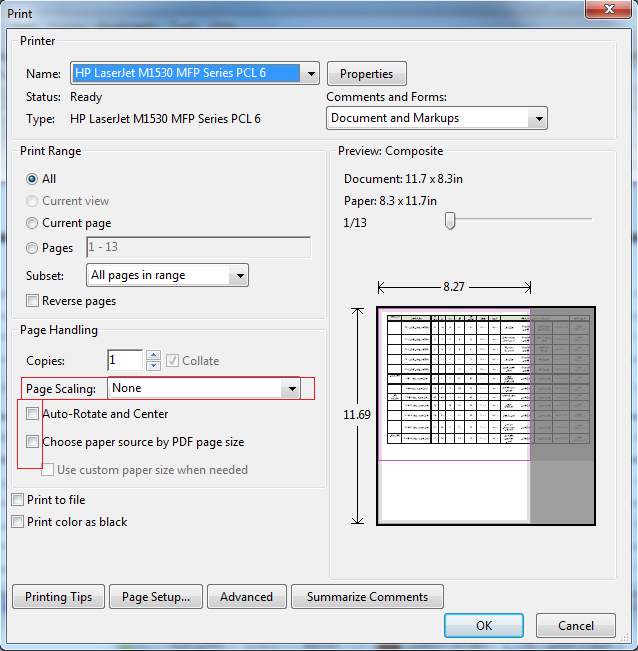
\includegraphics[width=0.6\textwidth]{Print-PDF}}}
     
    دقت کنید که بسته به پرینتر شما ممکن است موارد دیگری نظیر \lr{shrinking}  و غیره نیز 
    موجود باشد که باید همه غیر فعال شوند.
    با این ترتیب، مطمئناً حاشیه‌ها مطابق حاشیه‌ها در فایل پی‌دی‌اف خواهد بود.
    \section{اگر سوالی داشتیم، از چه کسی  بپرسیم؟}
    برای پرسیدن سوال‌های خود در مورد حروف‌چینی با زی‌پرشین،  می‌توانید به سایت‌های 
     \hbox{\href{http://qa.parsilatex.com}{ پرسش و پاسخ پارسی‌لاتک}}%
    \LTRfootnote{\url{http://qa.parsilatex.com}} 
    و یا 
    \hbox{\href{https://tex.stackexchange.com/questions}{\lr{Stack Exchange}}}%
    \LTRfootnote{\url{https://tex.stackexchange.com/questions}}
    مراجعه کنید. شما هم می‌توانید روزی به سوال‌های دیگران در این سایت جواب بدهید.
        

    \section{جمع‌بندی}
    در این فصل به بیان مقدمات نحوه استفاده از قالب پایان‌نامه/رساله دانشگاه قم پرداخته شد. 
    گرچه که مطالعه کامل این راهنما مقداری وقت شما را خواهد گرفت، اما مطمئن باشید از اتلاف وقت شما در ادامه کارتان تا حد زیادی جلوگیری خواهد کرد. 
    در نوشتن متن حاضر سعی شده است بیشتر مواردی که عموماً دانشجوان با آن مواجه هستند - و با نگاه ویژه به نیازهای دانشجویان ریاضی - ذکر شود. 
    در ادامه نوشتار نمونه مواردی از درج تصویر، نمودار، کد برنامه، الگوریتم، توضیحات، منابع، فرمول، تعریف، قضیه، مثال و جدول آمده است. 
    توصیه می‌شود یک کپی از کل فایل‌های این قالب را جداگانه از نسخه پایان‌نامه/رساله خود نگهداری نمایید تا در صورت نیاز بتوانید مراجعه فرمایید. 
    همچنین توصیه اکید داریم که رفع خطاهایی که احتمالاً با آن مواجه می‌شوید را به آخر موکول نفرمایید و به محض برخورد با خطا، آن را اشکال‌زدایی نموده و 
    خطا را برطرف فرمایید.
